\subsection{Ghantak}
\label{sec:specie-ghantak}

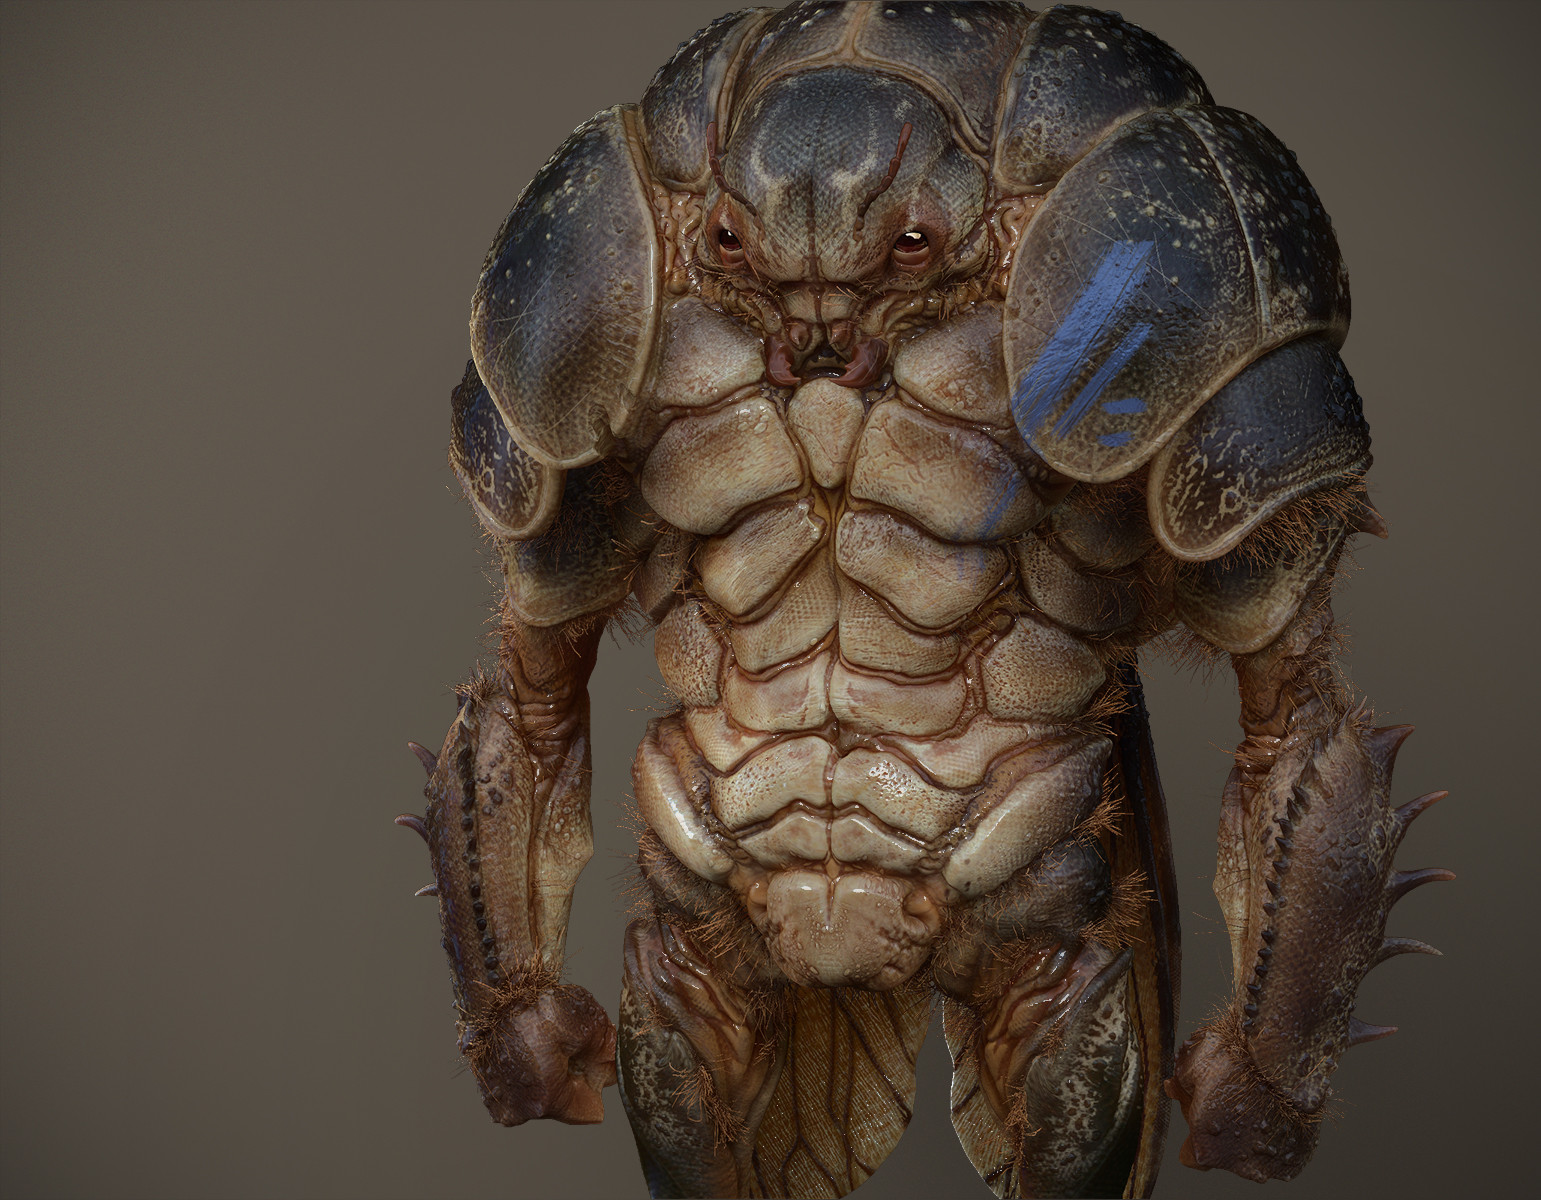
\includegraphics[width=\linewidth]{bruno-camara-beetle-brunocamara}

\begin{redtable}{\linewidth}{@{}L{.35}@{}L{.65}@{}}
  \textbf{Singular} & Ghan\\
  \textbf{Plural} & Ghantak\\
  \textbf{Height} & 135-170cm\\
  \textbf{Weight} & 55-90kg\\
  \textbf{Gender Ratio} & 90\% Genderless / 9\% Male / 1\% Female\\
  \textbf{Reproduction} & Ovuliparity (External egg fetilisation egg)\\
  \textbf{Maturity} & 5 years\\
  \textbf{Diet} & Herbivore\\
  \textbf{Homeworld} & Ghan\\
\end{redtable}

The Ghantak are an alien species evolved from the beetle-like insects native to their homeworld of Ghan. They are shorter than humans but weigh about the same, have an armoured carapace that covers their whole body, and their head is between the shoulders where the human chest would be. The odd placement for a Ghan head means that they must turn their whole body to look around.

Although each individual has their own free will, the Ghantak as a species have an innate tendancy to organise themselves into highly-structured hierachies. Most Ghan highly value honour and tradition, with personal sacrifice to uphold Ghantak values earning an individual glory and esteem. The race generally favours traditional solutions to problems, and individuals are uncomfortable when forced to exercise their own judgement.

While there used to be multiple independant hierarchies (each with their own Queen), the entire modern Ghantak society is now ruled by a singular Empress. The Empress is chosen from the Queens of the remaining hierarchies and she rules until her death.

To create a Ghan character, please refer to the \textit{\hyperref[sec:rules-creation]{Character creation section}}

\textbf{Ghantakian Names:}

Akiesuh, Bazoh, Bolbih, Choxu, Etix, Farqae, Gaknu, Graux, Greex, Havzal, Leksur, Mamobah, Mezuat, Semunu, Sydesih, Thonox, Vexoh, Zimla, Zouh, Ziuzoch

\textbf{Secondary Names:}

Ghantak do not take secondary names. Ghantakian first names are generally unique enough for a specific region. If pressed, the Ghantak will choose the next available incremental number for the region and their name.

\textbf{Males and Females:}

Females are especially reverred in Ghantakian culture, and are fanatically protected by all Ghantakians. They are rarely seen by non-Ghantakians, but can be differentiated by their large birthing pouch located just above their rectum. Males are also important to Ghantakian society, and usually are kept close to females to help breed the new generation. Males are allowed to travel the Black, and are almost indistinguishable from the genderless Ghantak (their genitalia is usually sheathed and protected by their carapace).
